\documentclass[conference]{IEEEtran}
\IEEEoverridecommandlockouts
% The preceding line is only needed to identify funding in the first footnote. If that is unneeded, please comment it out.
\usepackage{cite}
\usepackage{amsmath,amssymb,amsfonts}
\usepackage{algorithmic}
\usepackage{graphicx}
\usepackage{textcomp}
\usepackage{xcolor}
\usepackage{float}
\usepackage{cleveref}
\usepackage{epstopdf}
\def\BibTeX{{\rm B\kern-.05em{\sc i\kern-.025em b}\kern-.08em
    T\kern-.1667em\lower.7ex\hbox{E}\kern-.125emX}}


\DeclareMathOperator{\atantwo}{atan2}



\begin{document}

\title{Aarhus University MSc Course Project  \\ Control of Mobile Robots (AY 2019-20)}

\author{\IEEEauthorblockN{S. L. Skovgaard}
\IEEEauthorblockA{\textit{dept. of Engineering (of Aff.)} \\
\textit{Aarhus Unitversity (of Aff.)}\\
Aarhus, Denmark \\
201401682@post.au.dk}}

\maketitle

\begin{abstract}

The article will document how to develop control software for UAV's and simulate the controller using the popular Gazebo software. 	

\end{abstract}

\section{Introduction}
The main focus of this paper will be to explain and document the control software used to control a UAV robot. The software makes use of the robot operation system ROS. The paper will explain theory, code, simulation and results with accompanying figures and plots. The main objective of this project is to get a UAV to autonomously navigate to four coordinate-points.

\section{Theory}\label{theory}
\subsection{The Robot Operating System}
In order to develop software for robots in a structured and easy way, the robot operating system(ROS)\cite{ros} has been used for this project. ROS is based upon the subscriber-publisher pattern where nodes is able to publish data as topics and subscribe to specific topics. In this project a node has been developed that is a subscriber and publisher which enables the node to: gather data, make calculations using this data and the publish new data. Furthermore a another node has been made solely for the purpose of gathering data and displaying this data using different plots.

\subsection{PID-controller}
In the two tasks for this project will a PID-controller be implemented to control the Parrot Bebop2 drone. PID stands for proportional-integral-derivative controller. The proportional part of the controller acts as a linear feedback control system in which error correction is applied with a constant value that gives a proportional relationship between the measured value and the desired value. An increase in the $K_p$ parameter will result in a decrease in rise time and steady-state error as the current error will have bigger influence on the controller output. The negative side effect of an increase in $K_p$ is an increase in overshoot and small decrease in settling time as current error first becomes negative after the goal has been reached. The proportional control algorithm can be express mathematically as:


\begin{equation}
P_{out} = K_p e(t) \label{eq1}
\end{equation}

Where $P_{out}$ is the output of the controller, $K_p$ is the controller parameter, $e(t)$ is the measured error value at a certain time t. 

The integral part of the controller doesn't only look at the actual error as the proportional part does but also the time of which it has persisted. The integral part of the controller looks as at the past error, and if the applied force isn't enough to bring the error to zero, the force will be increased as time passes. An increase in the $K_i$ parameter will result in a decrease in rise time as the accumulated errors result in higher control output and it eliminates the steady-state error over time. The negative side effect of an increase in $K_i$ is an increase in overshoot and settling time as accumulated error first becomes smaller after the goal has been reached. The integral control algorithm can be express mathematically as:

\begin{equation}
I_{out} = K_i \int_{t}^{0}  e(\tau) d\tau \label{eq2}
\end{equation}

Where $I_{out}$ is the output of the controller, $K_i$ is the controller parameter, $e(\tau)$ is the error values from time 0 to the present time t. 

The derivative part of the controller look at the slope of the error over time and multiplies the rate of change by the derivative gain. The derivative part of the controller has an insight in the "future", for example if the object is quickly approaching the target, then the slope of the error over time will be negative will be negative and the controller output will decrease making sure the object doesn't overshoot by a lot. An increase in the $K_d$ parameter will result in overshoot and settling time as the slope of the error over time will result in a negative values as the object comes closer to the goal. An increase in $K_d$ doesn't have any notable influence in the rise time or the steady-state error. The derivative control algorithm can be express mathematically as:

\begin{equation}
D_{out} = K_d \frac{de(t)}{dt} \label{eq3}
\end{equation}

Where $D_{out}$ is the output of the controller, $K_d$ is the controller parameter, $de(t)$ is the change in error and  $dt$ is the change in time.

The by combining the three parts into a PID-controller it will be expressed mathematically as:
 
\begin{equation}
u(t) = K_p e(t)+ K_i \int_{t}^{0}  e(\tau) d\tau+K_d \frac{de(t)}{dt} \label{eq4}
\end{equation}

Where $u(t)$ is the controller output. 

\subsection{Coordinate transformation}
When working with unmanned aerial vehicles it is important to understand how the body of the aerial vehicle is oriented with respect to the earth.
The inertial frame is the earth-fixed set of axes that is used as an unmoving reference.  It is commonly known that the x-axis points north, the y-axis points east and the z-axis points below. This is also called North-East-Down (NED) reference frame. 
To move from the inertial frame to the body frame a sequence of rotations has to be performed. The sequence involve rotating the frame around one axis at the time. Before the first rotation the body reference coordinate matches that of the inertial frame. \\\\
\textit{First rotation: Yaw rotation}\\
The yaw rotation represents rotation about the z-axis by an angle $\psi$. This rotation generates a new coordinate frame where the z-axis of the body frame is aligned with the Z-axis of the inertial frame and x and y coordinate are rotated with the angle $\psi$. We call this transformation $T_\psi$. The rotation of inertial frame to $T_\psi$ frame is preformed be multiplying the vector by the rotation matrix see \cref{eq5} 

\begin{equation}
T_\psi=
\begin{bmatrix}
x_1\\
y_1\\
z_1 
\end{bmatrix}=
\begin{bmatrix}
cos(\psi) & sin(\psi) & 0\\
-sin(\psi) & cos(\psi) & 0 \\
0 & 0 & 1
\end{bmatrix}
\begin{bmatrix}
x_I\\
y_I\\
z_I 
\end{bmatrix}\label{eq5}
\end{equation}
\\\\
\textit{Second rotation: Yaw and Pitch rotation}\\
The second rotation involves rotating the newly generated frame $T_\psi$ Y-axis by an angle $\theta$. This rotation generates a new coordinate frame where the Y-axis of the new coordinate frame is aligned with the Y-axis of the $T_\psi$ frame and x and z coordinate are rotated with the angle $\theta$. This transformation is again performed by multiplying the vector by the rotation matrix see \cref{eq6}

\begin{equation}
T_\theta=
\begin{bmatrix}
x_2\\
y_2\\
z_2 
\end{bmatrix}=
\begin{bmatrix}
cos(\theta) & 0 & -sin(\theta)\\
0 & 1 & 0 \\
sin(\theta) & 0 & cos(\theta)
\end{bmatrix}
\begin{bmatrix}
x_1\\
y_1\\
z_1 
\end{bmatrix}\label{eq6}
\end{equation}
\\\\
\textit{Third rotation: Yaw, Pitch and Roll rotation}\\
The third rotation involves rotating the newly generated frame $T_\theta$ Y-axis by an angle $\phi$.
This rotation generates a new coordinate frame where the X-axis of the new coordinate frame is aligned with the X-axis of the $T_\theta$ frame and x and z coordinate are rotated with the angle $\phi$. We call this final frame the body frame. This transformation is again performed by multiplying the vector by the rotation matrix see \cref{eq7}
\begin{equation}
T_\phi=
\begin{bmatrix}
x_B\\
y_B\\
z_B 
\end{bmatrix}=
\begin{bmatrix}
1 & 0 & 0\\
0 & cos(\phi) & sin(\phi) \\
0 & -sin(\phi) & cos(\phi)
\end{bmatrix}
\begin{bmatrix}
x_2\\
y_2\\
z_2 
\end{bmatrix}\label{eq7}
\end{equation}
\\
The complete rotation matrix for moving from the inertial frame to the body frame is given by \cref{eq8}
\begin{equation}
T^B_I = T_\psi T_\theta T_\phi\label{eq8}
\end{equation}



\subsection{Parrot Bebop2 drone}
In order for the UAV to be able navigate to the given coordinates, a closed-loop control algorithm has to be developed in this case a p-controller is used to control the UAV. The UAV is a Parrot Bebob2 and is controlled using the package "bebop\_autonomy". By using this package it is possible to send velocity and angular velocity commands to a ROS topic and thereby control the speed and orientation of the drone. 

The p-controller developed in this project works by calculating the distance from the UAV to the currently active goal and use this as the error for the controller. A constant is multiplied to the error and the product of this will be used to set the velocity of the UAV.
  

\subsection{Gazebo}
Gazebo is simulation environment that works together with ROS and is therefore suitable as a simulation tool for this project. Parrot provides the Bebop2 UAV as a downloadable package for Gazebo and this package is used for this project.

\section{Python code}
The code used for this project is built using the rospy package which is a Python library. Roscpp is also available if C++ is preferred. 

As mentioned earlier in this article, ROS makes use of the publisher/subscribre pattern. A single node containing several classes have been made for this project. The classes are: p-controller, takeoff and plot\_maker. 

\textbf{P-controller:} The responsibility of p-controller is handle the calculations and navigation of the UAV. The error or the euclidean distance to the goal-coordinates is calculated by first calculating the distance in the x-plane then the y-plane and lastly the z-plane. This results in three different distances which all are used as the error in each axis. The error are multiplied a constant \textit{kp} and lastly the product of this is used to set the velocity in each direction, x, y and z.

\textbf{Takeoff:} As the name suggests this class handles the takeoff. It's a simple class that makes sure the drone has performed a complete takeoff sequence and when this is done it no longer has any responsibility. 

\textbf{Plot\_maker:} This class subscribes to the same topic as the p-controller class, /bebob/odom. It stores all values obtained from odometry and when the UAV has been to all goal-coordinates, displays a number of plots which will be discussed later in the article. 


One task for this project is to navigate to the four goals with a set yaw angle, this however haven't been completed here as the author has no idea how the rotation matrices are supposed to be programmed. 

\section{Results and discussion}


\subsection{Simulation results}
To verify that the controller behaves as expected and to ensure that the drone will not crash when testing in real life, the controller has been tested in simulation first. The behaviour should be more or less the same when testing in a real world scenario. The simulation tests covers both the hovering and waypoint scenario however, only the waypoint scenario will be shown in this report for the simulation. The drone used for the simulation as well as in the real world is the Parrot bebop2 UAV.

The goal for the controller has been to optimize for speed which means that it is allowed to have a relative high amount of overshoot. Furthermore it should have a quick settling time as this has a big impact on how quick the drone will complete its waypoint task. To accommodate for these requirements manual tuning of the three controller coefficients found a reasonably well suited controller with the values set to: Kp = 0.1, Ki = 0.01 and Kd = 0.1. On \cref{fig:sim_pos} the x, y and z position of the drone can be seen when using this controller. This result is a good start for the real world scenario and will be tuned further for the waypoint task.

\begin{figure}[hbtp]
	\centering
	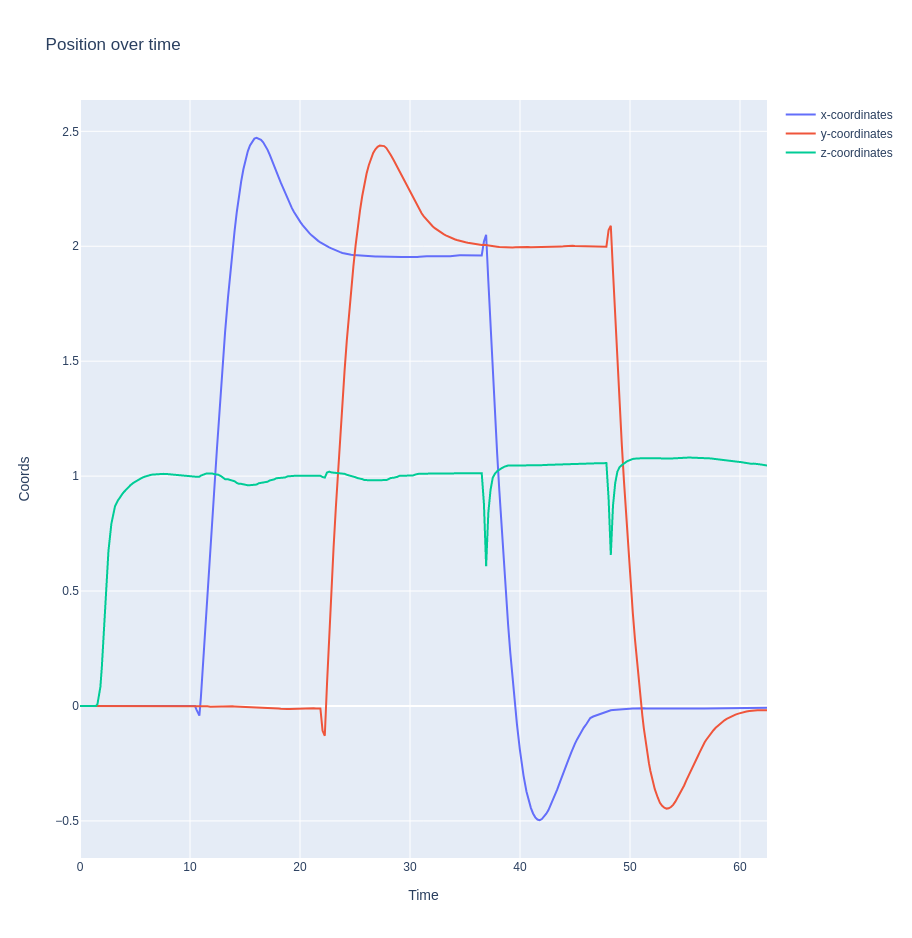
\includegraphics[width=1.0\linewidth]{images/task2_sim_pos.png}
	\caption{x, y and z coordinates of the drone in simulation. (Kp = 0.1, Ki = 0.01, Kd = 0.1)}
	\label{fig:sim_pos}
\end{figure}

Another way to visualize the simulation is using the program rviz which makes is possible to display the orientation as well as the position in 3D space. This can be seen on \cref{fig:sim_rviz}. On this figure it is also apparent that the yaw angle is constant for the drone at all times. When observing the behaviour on \cref{fig:sim_rviz} the controller was again verified to be a good start for the real world scenario.

\begin{figure}[hbtp]
	\centering
	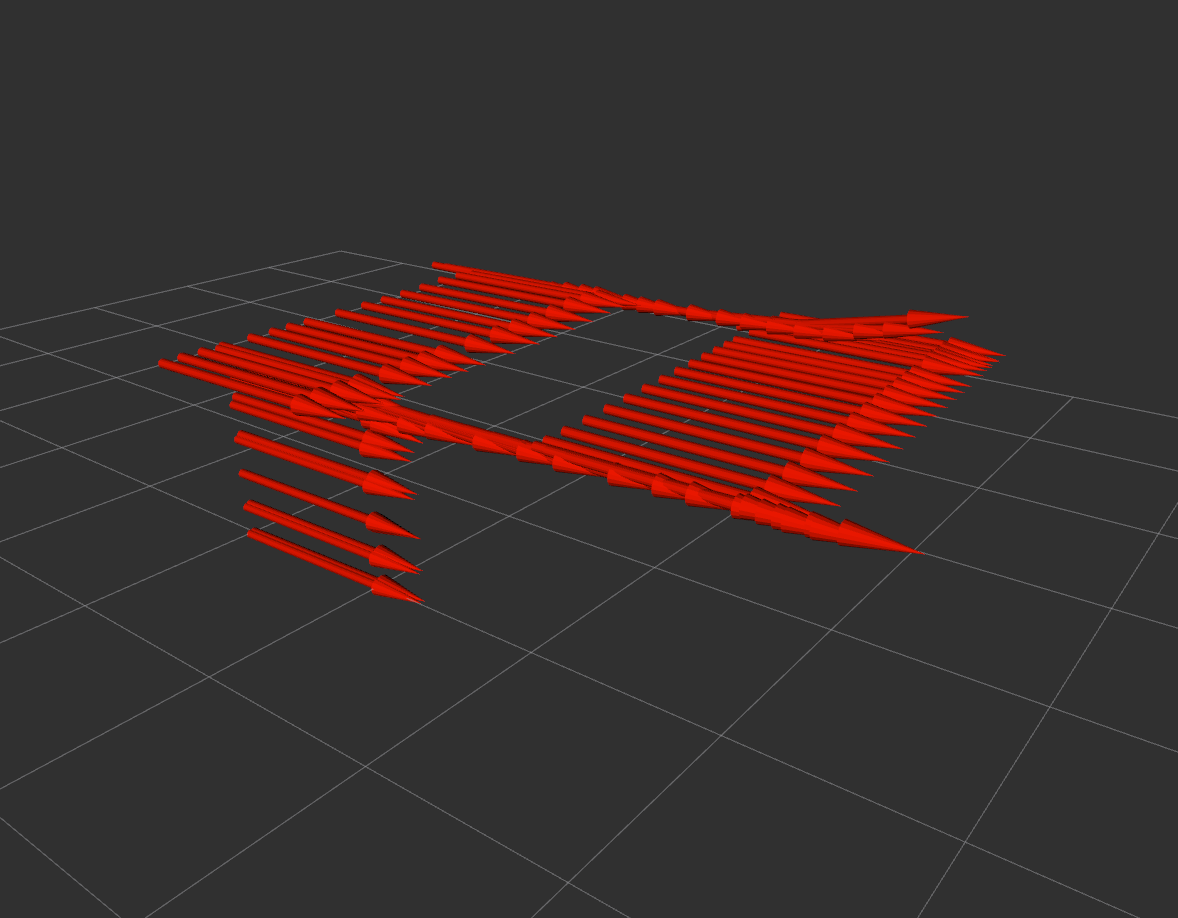
\includegraphics[width=1.0\linewidth]{images/task2_sim_rviz.png}
	\caption{x, y and z coordinates of the drone in simulation. (Kp = 0.1, Ki = 0.01, Kd = 0.1)}
	\label{fig:sim_rviz}
\end{figure}

\subsection{Real world results}
After having tested the controller in simulation the next step is to test it in a real world scenario. This is done using the Vicon motion control system which is able to accurately measure a UAV's position. This is done through 12 motion capture cameras that can locate small grey balls which are taped onto the drone itself. The Vicon system uses these balls as an reference point in space which can then be grouped together in the Vicon software and it will be able to publish the position as a topic in ROS. This means that the controller will now subscribe to this topic instead of the odometry data from the UAV itself.

The first task is to get the UAV to hover and be able to withstand disturbances. This means that if the drone experiences large gushes of wind it will be able to go back to its original position autonomously. To simulate this disturbance a piece of string was tied to the UAV and a person would simply pull in the string.

On \cref{fig:task1_10_pos} the drone is set to hover at position (0, 0, 1). The controller is the same as in simulation (Kp = 0.1, Ki = 0.01, Kd = 0.1). It can be seen how the UAV flies to the desired location and then a big disturbance occurs which displaces the UAV over 2.5 meters in the negative x-direction. However the UAV quickly recovers and converges to its original position.  

\begin{figure}[hbtp]
	\centering
	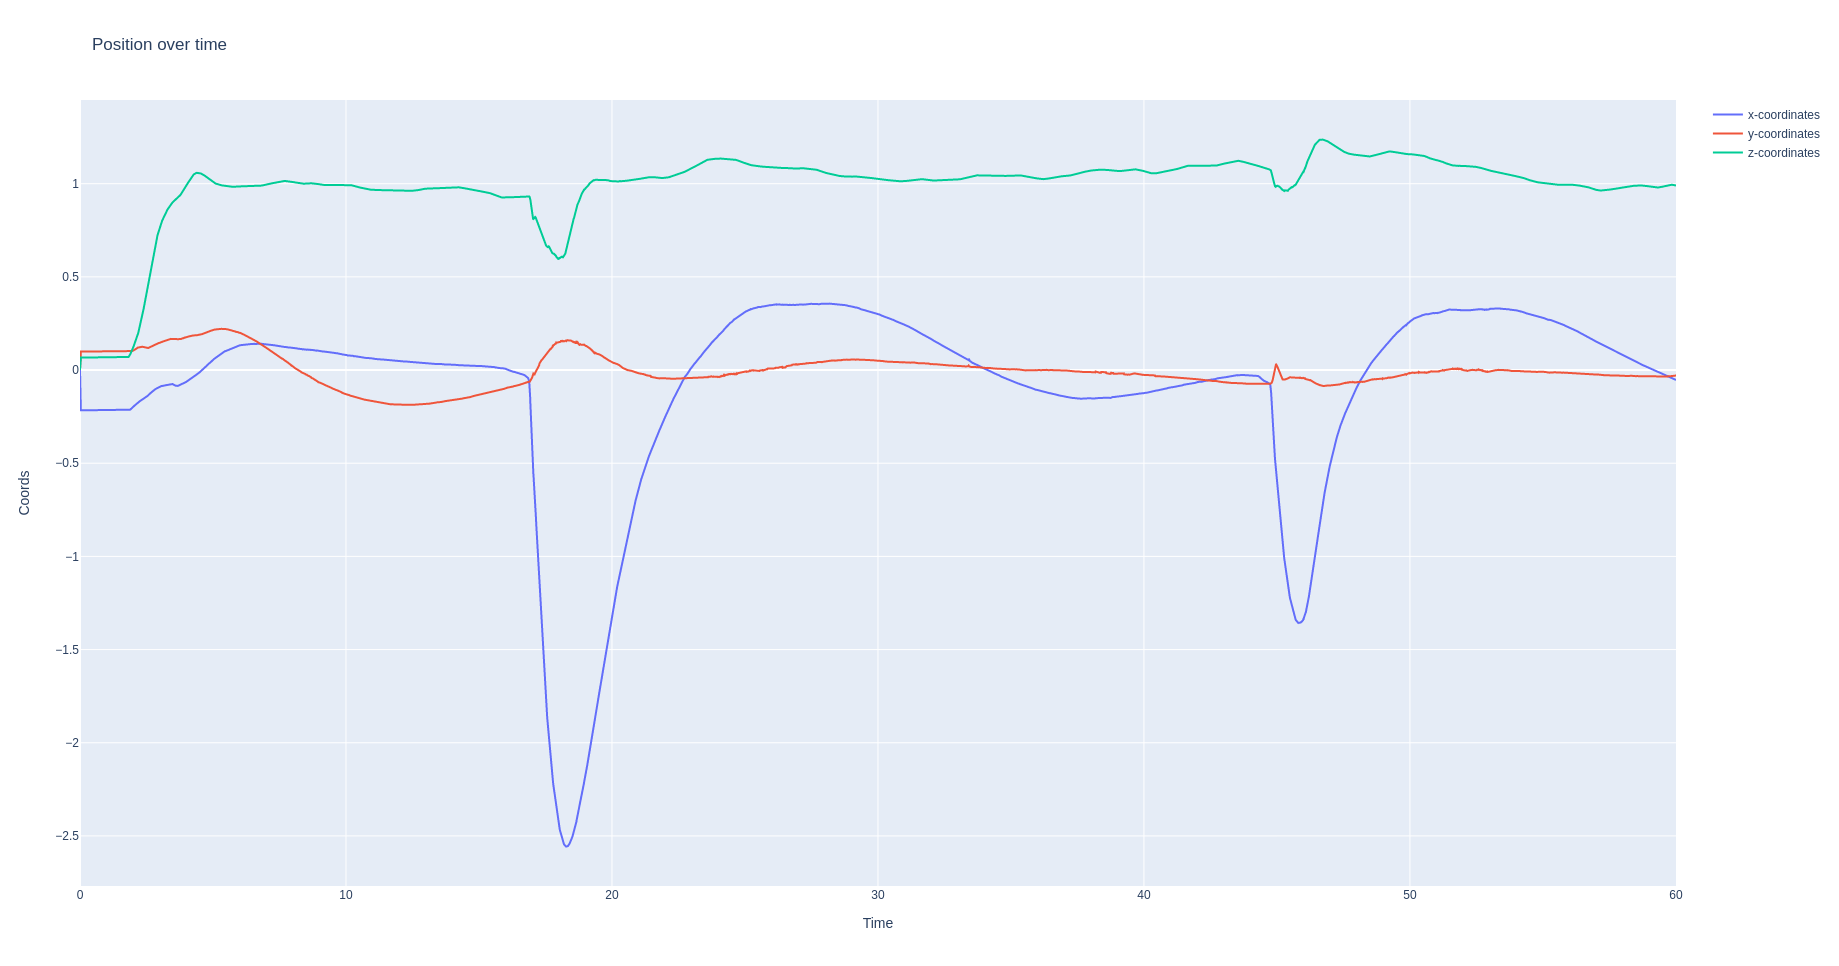
\includegraphics[width=1.0\linewidth]{images/task1_10_pos.png}
	\caption{x, y and z coordinates of the UAV in the hovering scenario. (Kp = 0.1, Ki = 0.01, Kd = 0.1)}
	\label{fig:task1_10_pos}
\end{figure}

On \cref{fig:task1_10_err} the same behaviour can be seen. When the disturbance occurs there is a big spike in the error which is expected. 

\begin{figure}[hbtp]
	\centering
	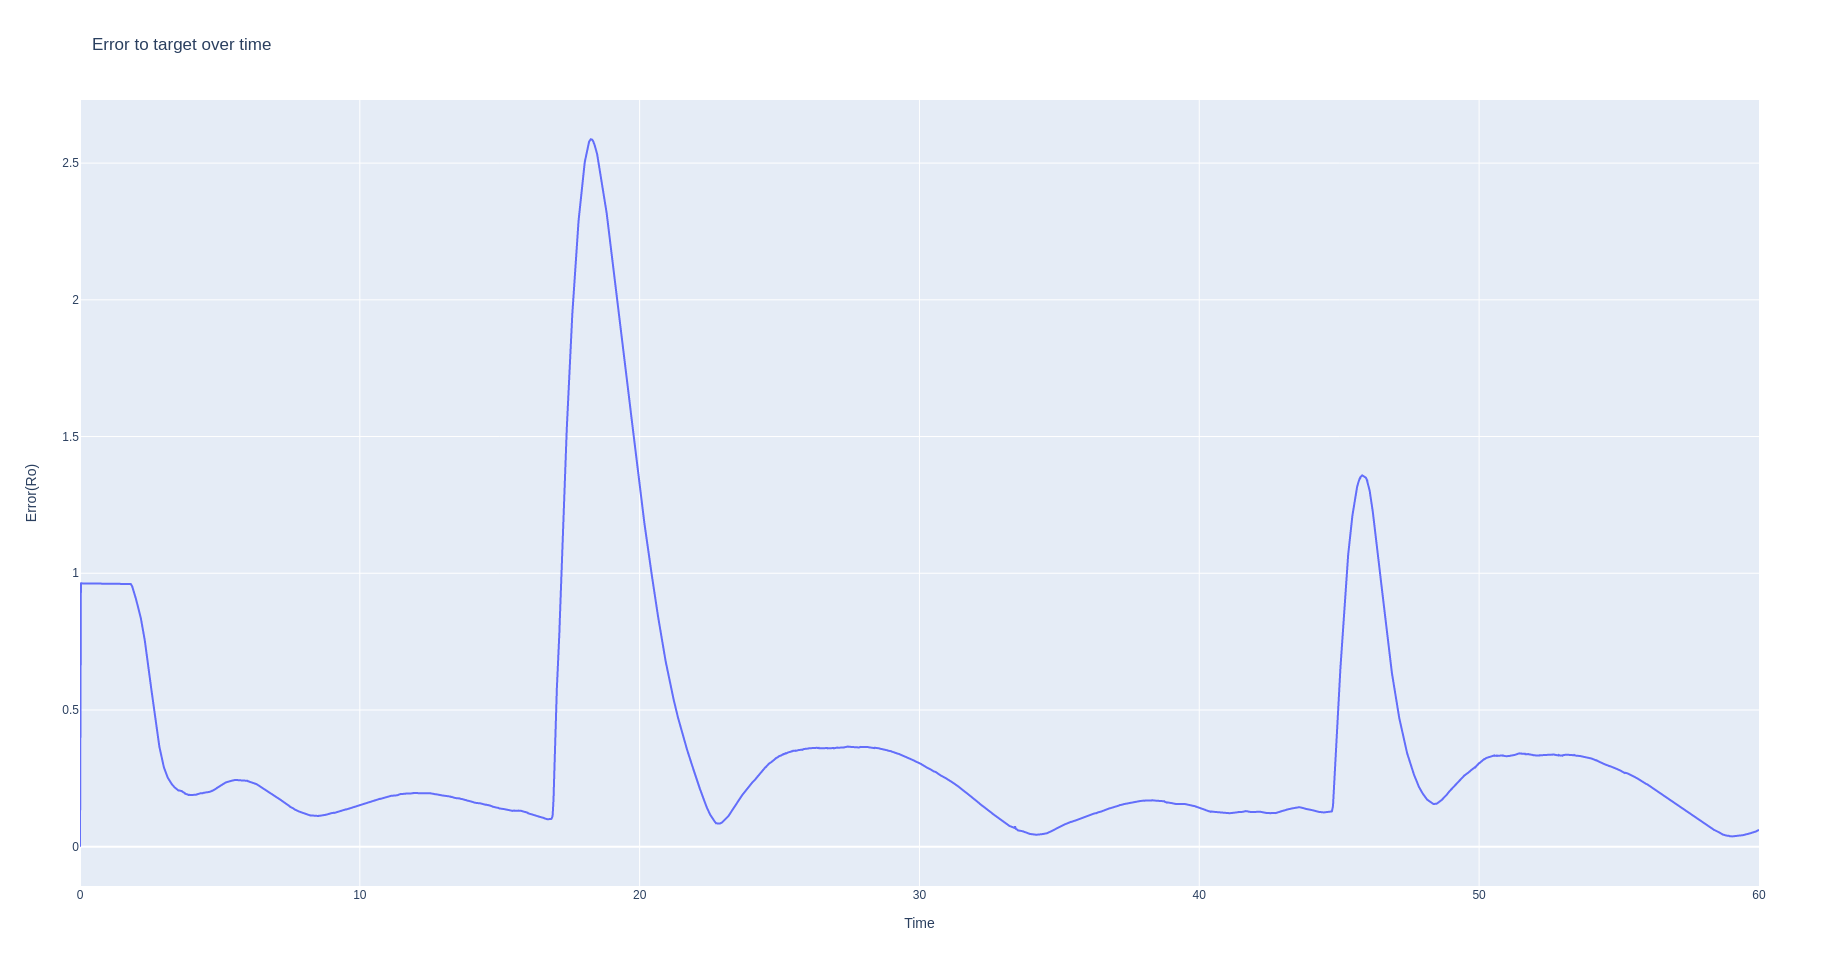
\includegraphics[width=1.0\linewidth]{images/task1_10_err.png}
	\caption{Error(distance) to target(0,0,1). (Kp = 0.1, Ki = 0.01, Kd = 0.1)}
	\label{fig:task1_10_err}
\end{figure}

The controller used on \cref{fig:task1_10_err} and \cref{fig:task1_10_pos} seems to be doing a good job, however it also looks like it can be improved. By tuning the value of Kd the overshoot should decrease and in turn make it settle quicker which is one of the requirements for this controller. On \cref{fig:task1_11_pos} the position of the UAV can be seen. Kd has been increase threefold and now the overshoot has decreased greatly and it settles quicker. It still looks like there is some overshoot but it was observed during the test that the string attached to the UAV cause some amount of drag and made the UAV move slightly slower causing this overshoot from t=25 to t=43.

\begin{figure}[hbtp]
	\centering
	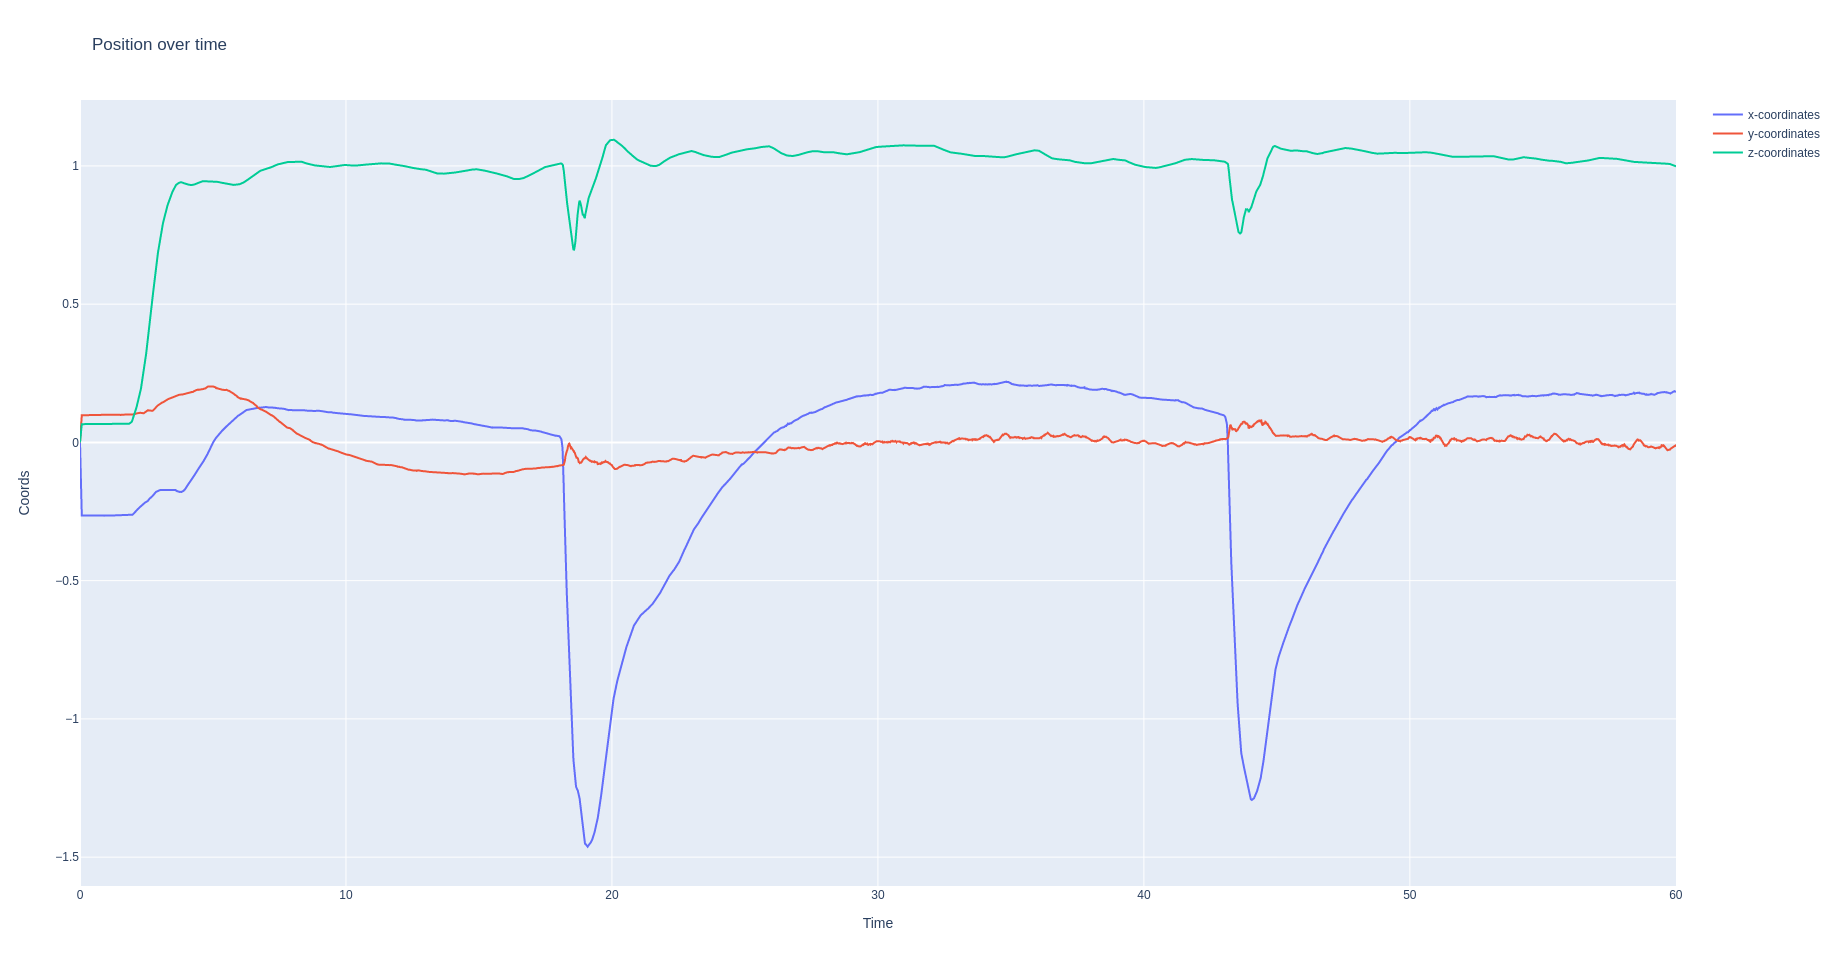
\includegraphics[width=1.0\linewidth]{images/task1_11_pos.png}
	\caption{x, y and z coordinates of the UAV. (Kp = 0.1, Ki = 0.01, Kd = 0.3)}
	\label{fig:task1_11_pos}
\end{figure}

On \cref{fig:task1_11_err} the error to the target can be seen. It shows the same drawn out overshoot caused by the strings weight and drag on the floor.

\begin{figure}[hbtp]
	\centering
	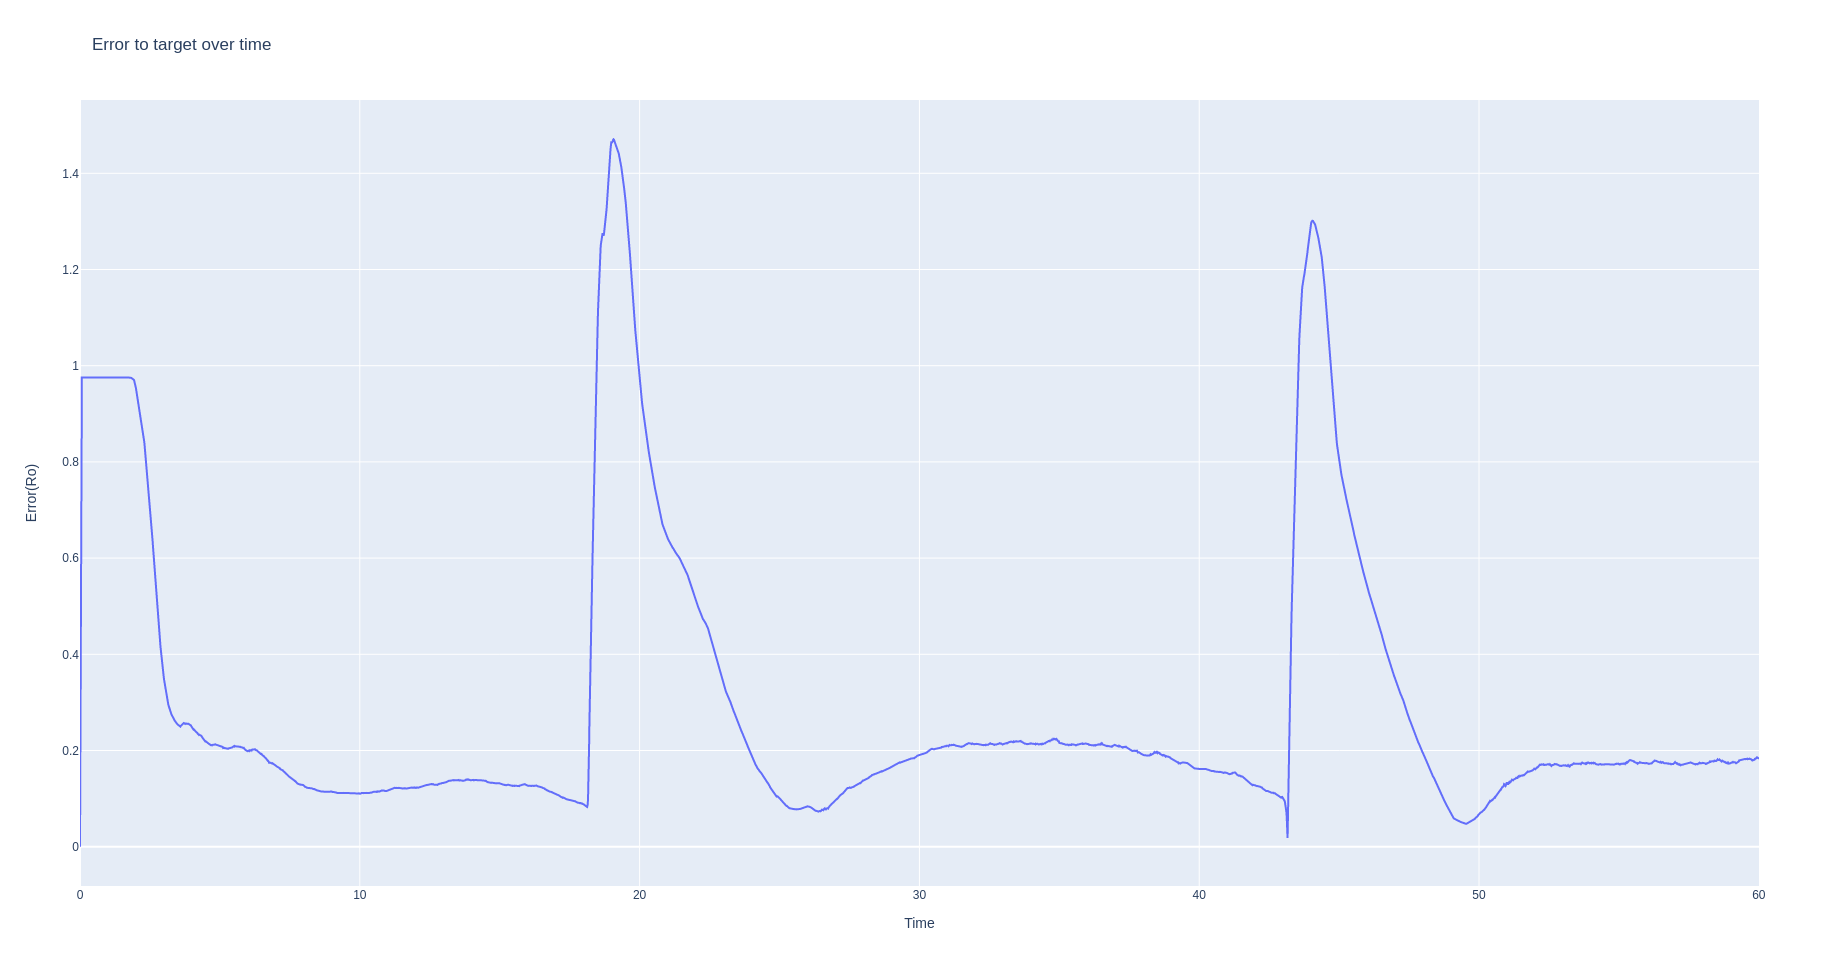
\includegraphics[width=1.0\linewidth]{images/task1_11_err.png}
	\caption{Error(distance) to target(0,0,1). (Kp = 0.1, Ki = 0.01, Kd = 0.3)}
	\label{fig:task1_11_err}
\end{figure}

To decrease the rise time and eliminate the steady state error an increase in Ki will help alleviate that. This comes with a cost of an increase in settling time and decreases the stability which goes against the requirements for this controller. A controller with a Ki=0.03 has been tested and shows that the UAV takes a big hit to the settling time. These figures can be seen in appendix A.

When tuning the proportional term of the controller the rise time should decrease and the overshoot should increase, however the settling time will increase and the stability will decrease. On \cref{fig:task1_4_pos} it can be seen how the overshoot is increase compared to \cref{fig:task1_10_pos} and the stability has been decreased. 

\begin{figure}[hbtp]
	\centering
	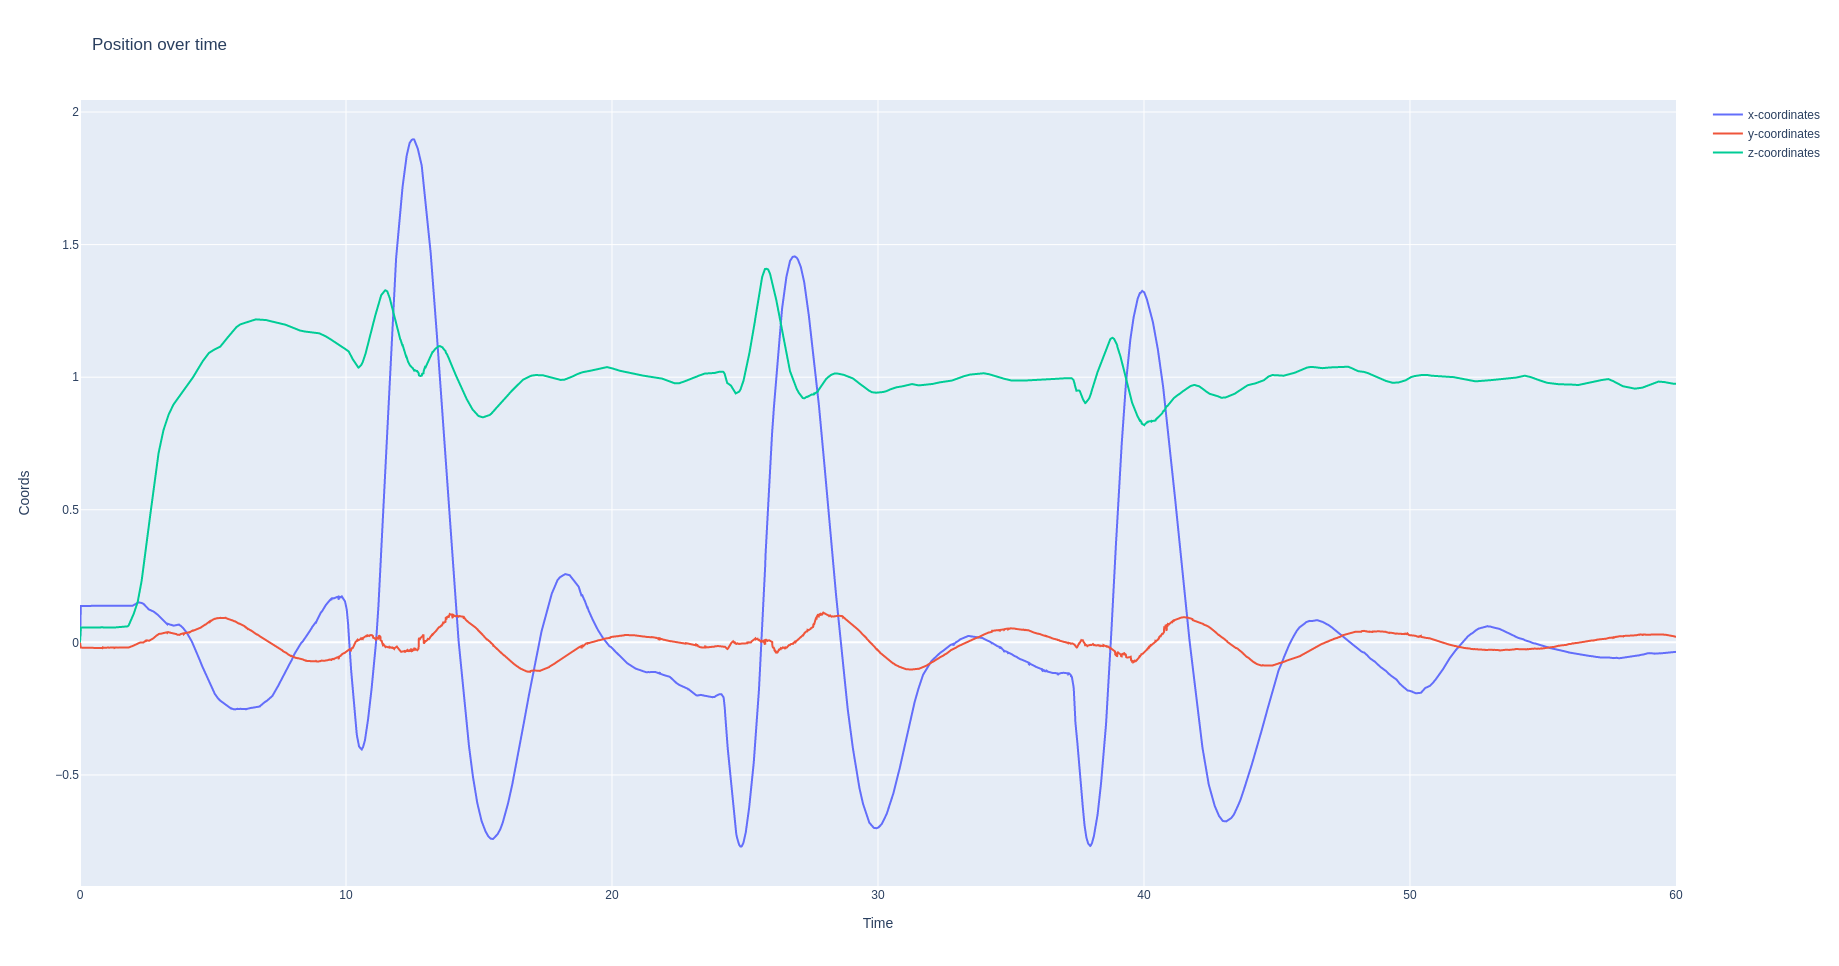
\includegraphics[width=1.0\linewidth]{images/task1_4_pos.png}
	\caption{x, y and z coordinates of the UAV. (Kp = 0.3, Ki = 0.01, Kd = 0.1)}
	\label{fig:task1_4_pos}
\end{figure}

The overshoot and stability issues can also be seen on \cref{fig:task1_4_err}. 
\begin{figure}[hbtp]
	\centering
	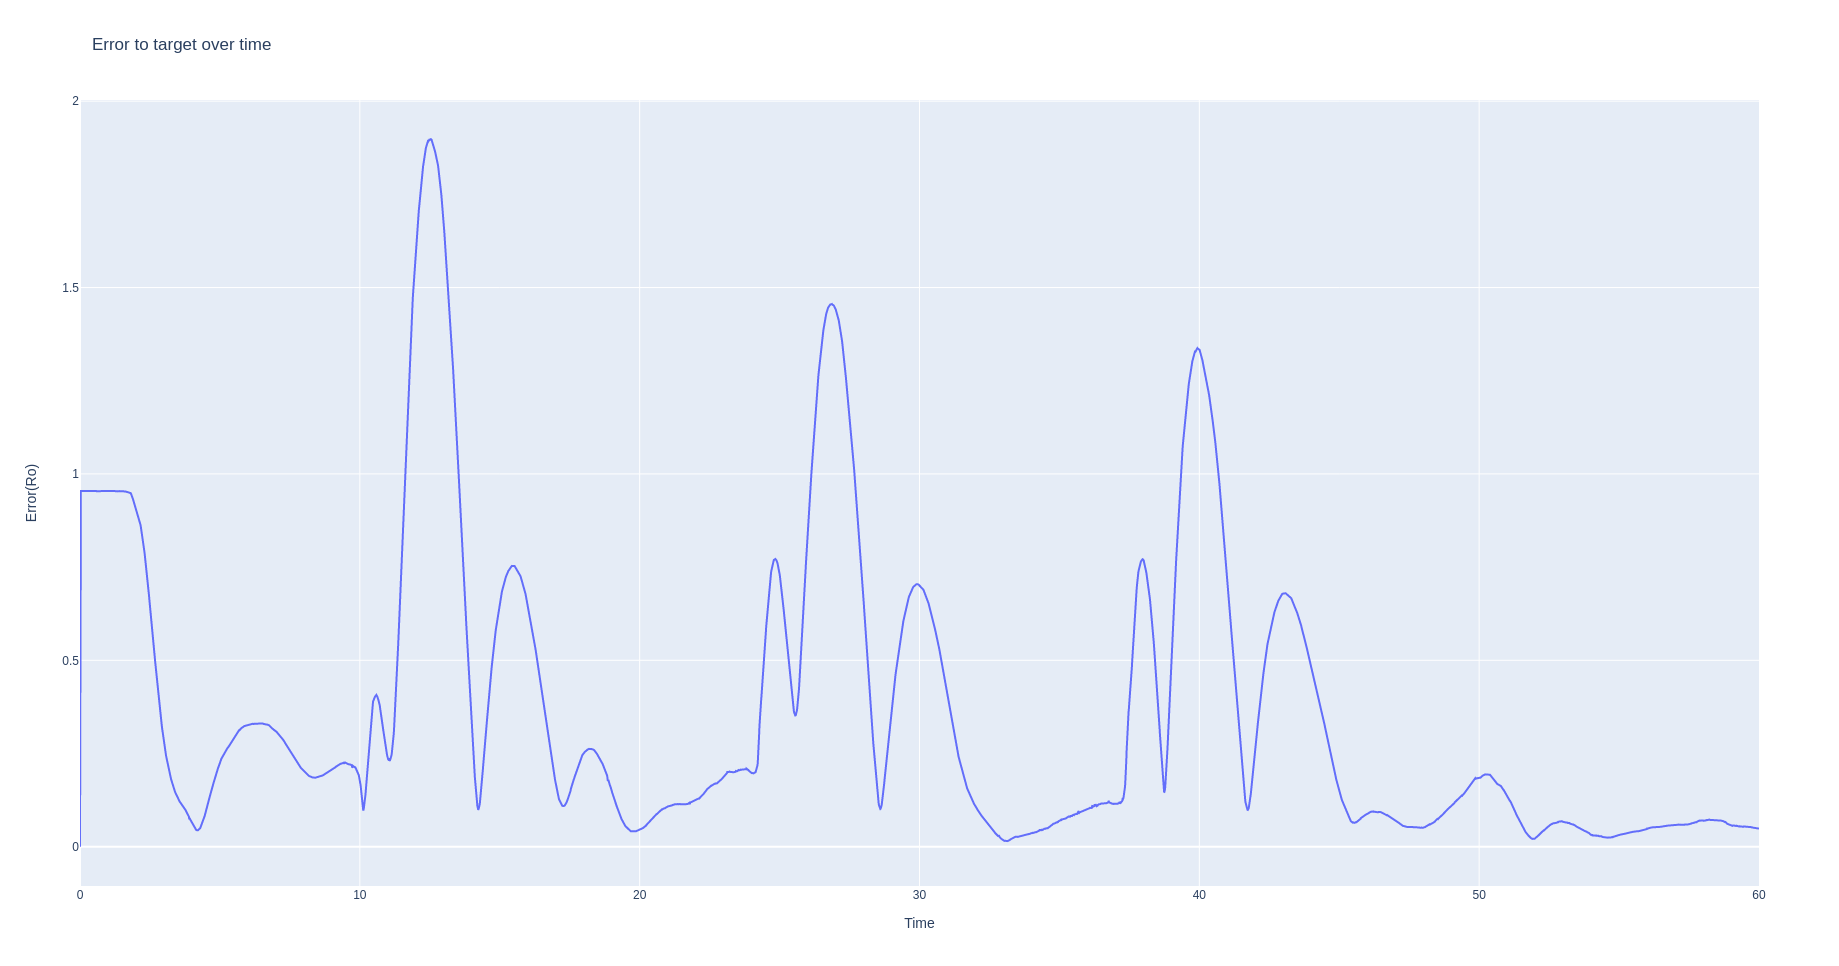
\includegraphics[width=1.0\linewidth]{images/task1_4_err.png}
	\caption{Error(distance) to target(0,0,1). (Kp = 0.3, Ki = 0.01, Kd = 0.3)}
	\label{fig:task1_4_err}
\end{figure}

When examining all of these plots it is apparent that a PID controller is needed. After some manual tuning the parameters for this controller was found to be Kp = 0.4, Ki= 0.02 and Kd=0.4. By using the proportional, integral and derivative part it is possible to cancel out the negative aspects of each term. This controller can be seen on \cref{fig:task1_9_pos}. There is a significant amount of jitter when looking at the y-axis. This was observed in multiple tests and only occurred when the UAV was in a certain location. This could indicate a problem with the Vicon system or a problem with the motion capture system unable to locate all the balls taped onto the UAV. Whenever the UAV moved out this area the jitter disappeared and it performed as expected. This jitter can be seen on \cref{fig:task1_9_pos} and \cref{fig:task1_9_err} at t=15 and t=35.

\begin{figure}[hbtp]
	\centering
	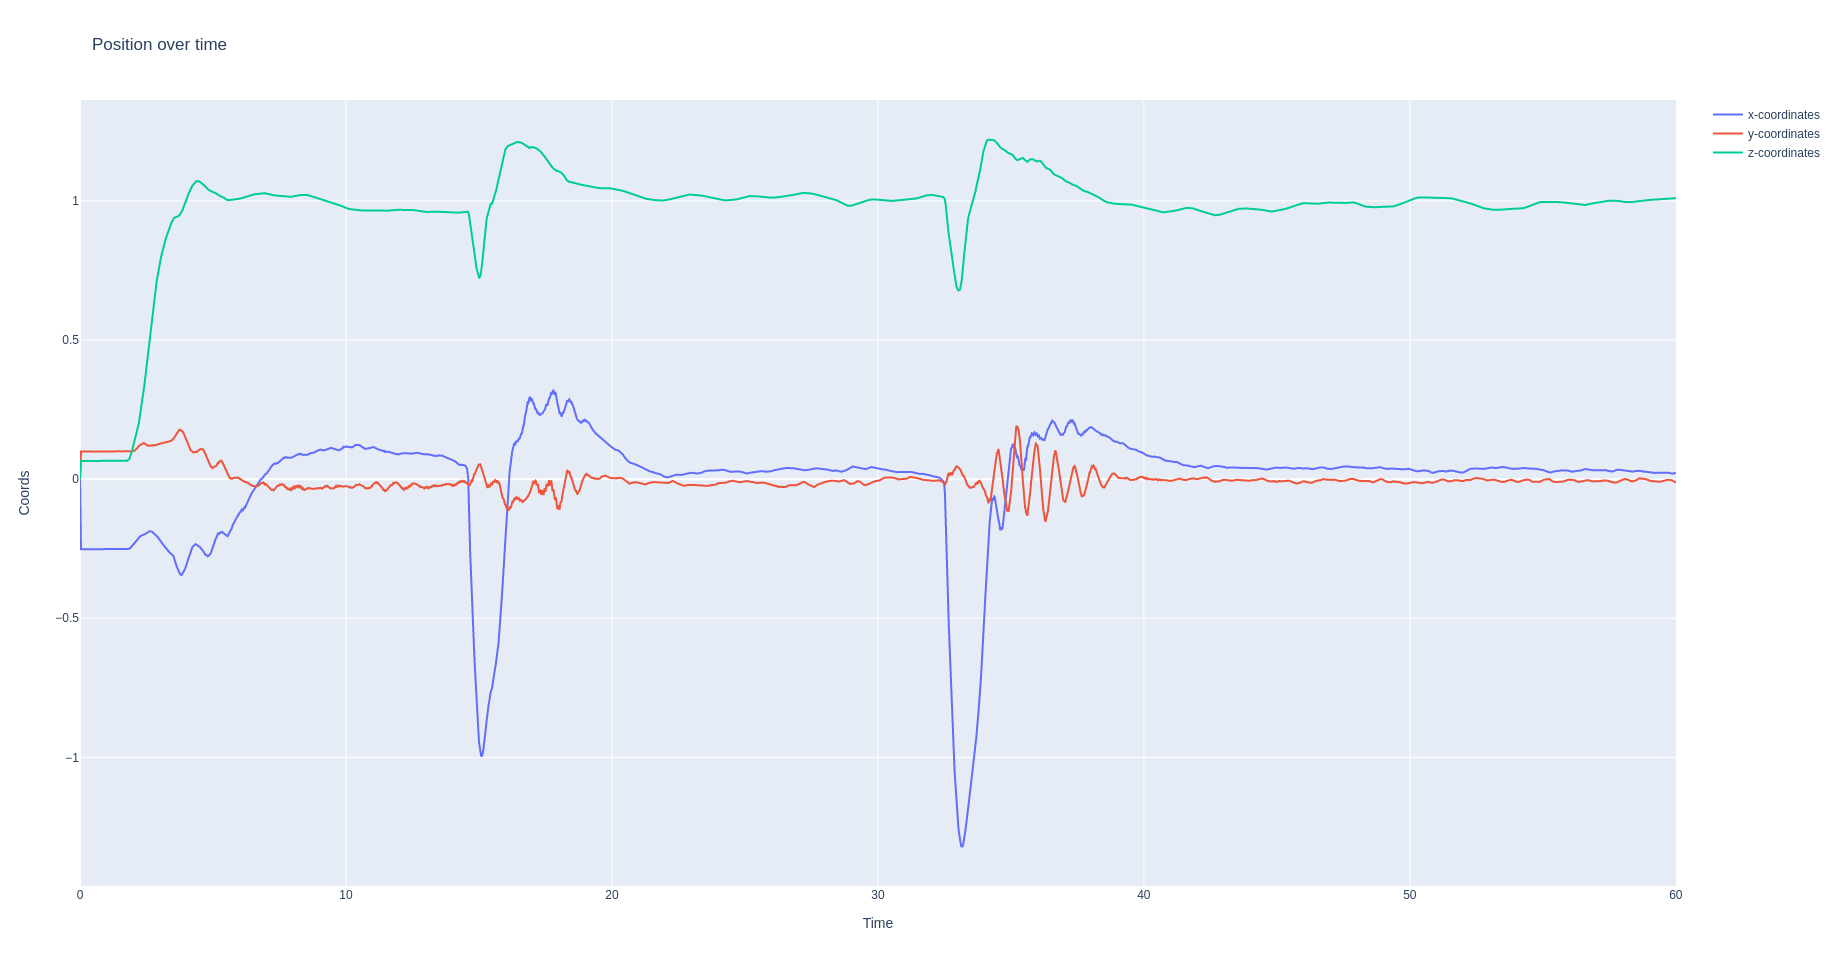
\includegraphics[width=1.0\linewidth]{images/task1_9_pos.png}
	\caption{x, y and z coordinates of the UAV. (Kp = 0.4, Ki = 0.02, Kd = 0.4)}
	\label{fig:task1_9_pos}
\end{figure}

\begin{figure}[hbtp]
	\centering
	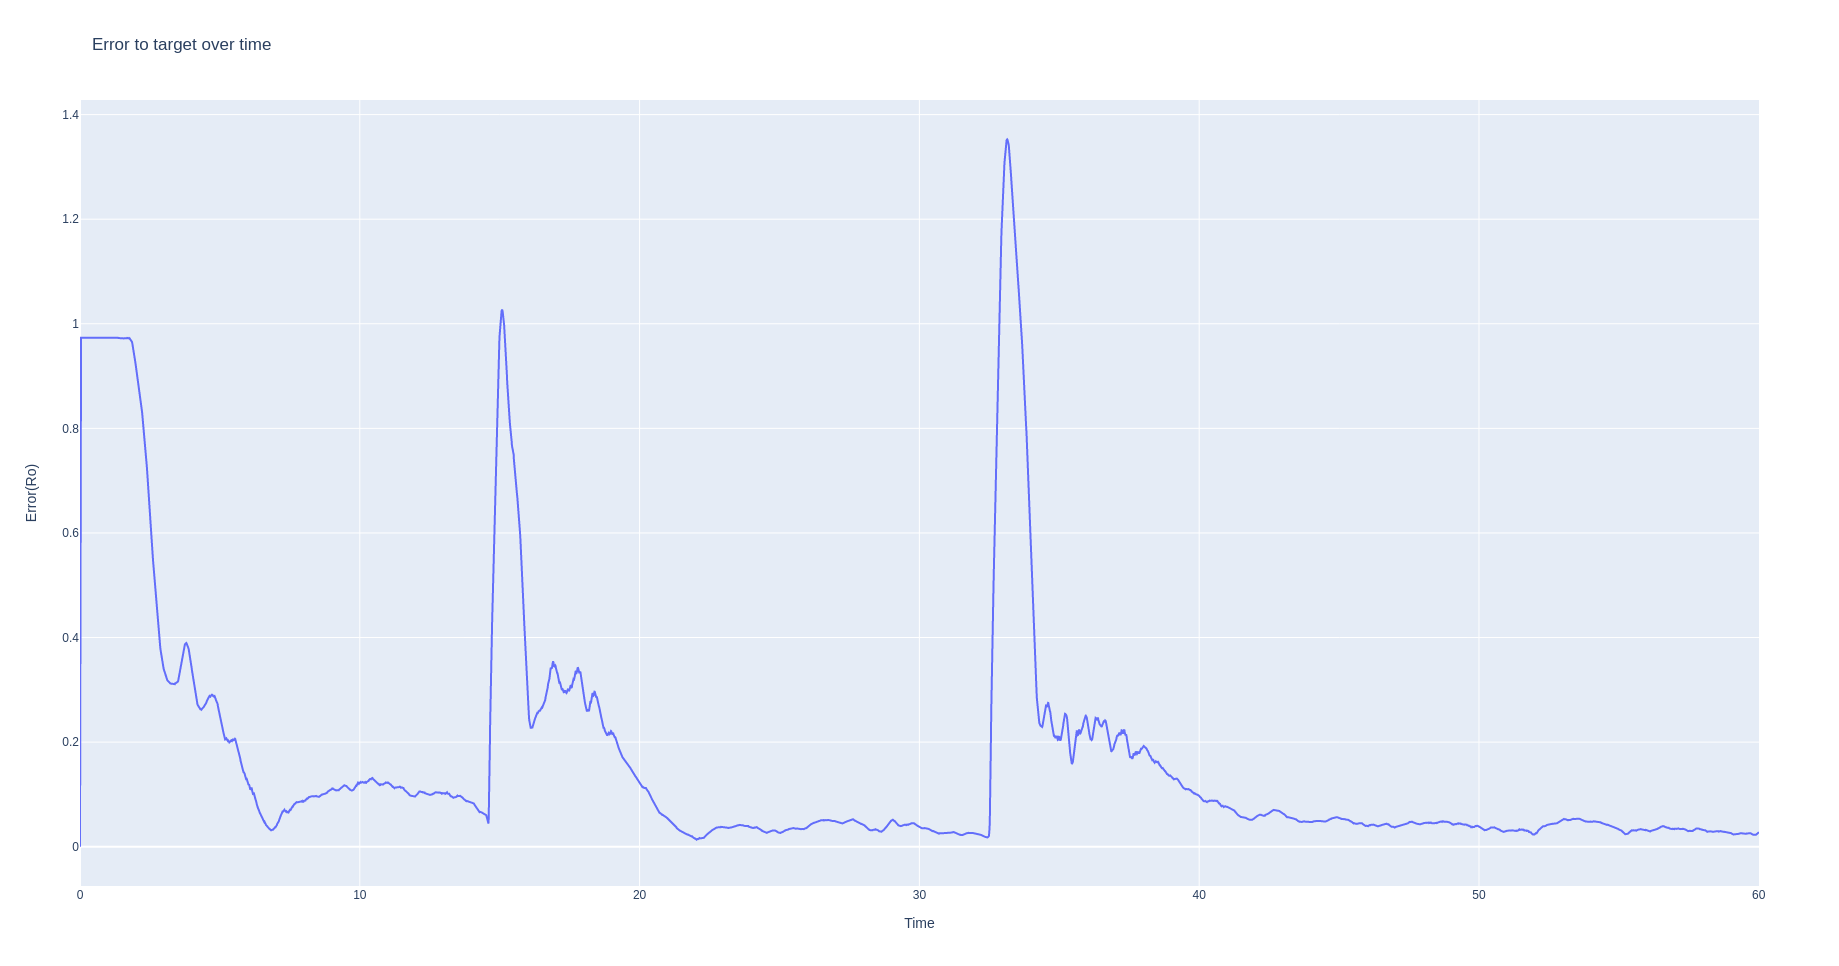
\includegraphics[width=1.0\linewidth]{images/task1_9_err.png}
	\caption{x, y and z coordinates of the UAV. (Kp = 0.4, Ki = 0.02, Kd = 0.4)}
	\label{fig:task1_9_err}
\end{figure}

Based on the last two figures a very quick and stable controller has been made and it meets the requirement of having a quick settling time.

\section{Conclusion}
The main objective for this project has been to develop control software for a UAV so it would be able to navigate to four coordinate-points in 3D space. The plots shown during the Results and discussion section have clearly shown how the UAV reaches the four points. Furthermore different tools for analysing the UAV data have been used such as rviz. Task 2 haven't been completed because of time constraints and would have high priority for future work.

\begin{thebibliography}{00}

\bibitem{ros} http://wiki.ros.org/, date: 3/10/2020

\bibitem{Week3} Erdal Kaycan, ``Control Of Mobile Robots, week 3: Ground Robot models``, 16th of September 2020

\bibitem{book} RANDAL W. BEARD and TIMOTHY W. McLAIN, SMALL UNMANNED AIRCRAFT Theory and Practice, 2012

\end{thebibliography}
\vspace{12pt}

\end{document}
